\documentclass[platex]{jsarticle}
\usepackage[dvipdfmx]{graphicx}
\usepackage{here}
%\renewcommand{\labelenumi}{(\arabic{enumi})}
\usepackage[RPvoltages]{circuitikz}
\usepackage{siunitx}

\begin{document}
% ここから本文

\begin{figure}[H]
	\centering
	% 図4.4
	\begin{circuitikz}
		\ctikzset{quadpoles/transformer core/inner=1, quadpoles/transformer core/width=0.6}
		% ==============
		%  電源
		% ==============
		\draw
		(0,0) to [sV] (0,3)
		(-1.2,1.5) node [anchor=west] {FG}
		(1.2,1.5) node [anchor=east] {$V_\mathrm{in}$}
		;
		% ==============
		%  RC直列
		% ==============
		\draw (0,3)
		to [european resistor = $R$] (3,3)
		to [C = $C$, *-] (3,0)
		to [short, *-] (0,0)
		;
		% ==============
		%  node 管理
		% ==============
		\draw
		(3,3) to [short, -o] (4.5,3)
		(3,0) to [short, -o] (4.5,0)
		(3,0) node [cground] {}
		;
		% ==============
		%  Vc
		% ==============
		\draw[<->=latex]
		(4,2.8) to [] (4,0.2)
		;
		\draw
		(4,1.5) node [anchor=west] {$V_\mathrm{C}$}
		;
	\end{circuitikz}
	\caption{ローパスフィルタ回路}
	\label{fig4.4}
\end{figure}


\begin{figure}[H]
	\begin{minipage}{0.49\hsize}
		\centering
		% 図4.1
		% 左図
		\begin{circuitikz}
			\ctikzset{quadpoles/transformer core/inner=1, quadpoles/transformer core/width=0.6}
			% ==============
			%  電源
			% ==============
			\draw
			(0,4) to [battery1] (0,0)
			(0,4) to [nos] (3,4)
			to [short] (4,4)
			(-1.2,2) node [anchor=west] {FG}
			(1.2,2) node [anchor=east] {$V_\mathrm{in}$}
			;
			% ==============
			%  RC直列
			% ==============
			\draw (4,4)
			to [european resistor = $R$] (4,2)
			to [C = $C$] (4,0)
			to [short] (0,0)
			;
			% ==============
			%  i 矢印
			% ==============
			\draw[->, >=stealth]
			([shift={(1.5,2)}]90:1.5) arc[radius=1.5, start angle=90, end angle=-90]
			;
			\draw
			(2.5,2) node [anchor=east] {$i$}
			;
		\end{circuitikz}
		\label{LowPass}
	\end{minipage}
	\begin{minipage}{0.49\hsize}
		\centering
		% 右図
		\begin{circuitikz}
			\ctikzset{quadpoles/transformer core/inner=1, quadpoles/transformer core/width=0.6}
			% ==============
			%  電源
			% ==============
			\draw
			(0,0) to [sqV] (0,4)
			(-1.2,2) node [anchor=west] {FG}
			(1.2,2) node [anchor=east] {$V_\mathrm{in}$}
			;
			% ==============
			%  RC直列
			% ==============
			\draw (0,4)
			to [short] (4,4)
			to [european resistor = $R$] (4,2)
			to [C = $C$] (4,0)
			to [short] (0,0)
			;
			% ==============
			%  i 矢印
			% ==============
			\draw[->, >=stealth]
			([shift={(1.5,2)}]90:1.5) arc[radius=1.5, start angle=90, end angle=-90]
			;
			\draw
			(2.5,2) node [anchor=east] {$i$}
			;
		\end{circuitikz}
	\end{minipage}
	\caption{RC直列回路の過渡応答(充電過程)}
	\label{fig4.1}
\end{figure}


\begin{figure}[H]
	% 図4.2
	\begin{minipage}{0.49\hsize}
		\centering
		% 図4.1
		% 左図
		\begin{circuitikz}
			\ctikzset{quadpoles/transformer core/inner=1, quadpoles/transformer core/width=0.6}
			% ==============
			%  電源
			% ==============
			\draw
			(0,4) to [battery1] (0,0)
			(0,4) to [nos] (3,4)
			to [short] (4,4)
			(-1.2,2) node [anchor=west] {FG}
			(1.2,2) node [anchor=east] {$V_\mathrm{in}$}
			;
			% ==============
			%  RC直列
			% ==============
			\draw (4,4)
			to [european resistor = $R$] (4,2)
			to [C = $C$] (4,0)
			to [short] (0,0)
			;
			% ==============
			%  i 矢印
			% ==============
			\draw[->, >=stealth]
			([shift={(1.5,2)}]-90:1.5) arc[radius=1.5, start angle=-90, end angle=90]
			;
			\draw
			(2.5,2) node [anchor=east] {$i$}
			;
		\end{circuitikz}
	\end{minipage}
	\begin{minipage}{0.49\hsize}
		\centering
		% 右図
		\begin{circuitikz}
			\ctikzset{quadpoles/transformer core/inner=1, quadpoles/transformer core/width=0.6}
			% ==============
			%  電源
			% ==============
			\draw
			(0,0) to [sqV] (0,4)
			(-1.2,2) node [anchor=west] {FG}
			(1.2,2) node [anchor=east] {$V_\mathrm{in}$}
			;
			% ==============
			%  RC直列
			% ==============
			\draw (0,4)
			to [short] (4,4)
			to [european resistor = $R$] (4,2)
			to [C = $C$] (4,0)
			to [short] (0,0)
			;
			% ==============
			%  i 矢印
			% ==============
			\draw[->, >=stealth]
			([shift={(1.5,2)}]-90:1.5) arc[radius=1.5, start angle=-90, end angle=90]
			;
			\draw
			(2.5,2) node [anchor=east] {$i$}
			;
		\end{circuitikz}
	\end{minipage}
	\caption{RC直列回路の過渡応答(放電過程)}
	\label{fig4.2}
\end{figure}


\begin{figure}[H]
	\centering
	% 図4.4
	\begin{circuitikz}
		\ctikzset{quadpoles/transformer core/inner=1, quadpoles/transformer core/width=0.6}
		% ==============
		%  電源
		% ==============
		\draw
		(0,0) to [sV] (0,3)
		(-1.2,1.5) node [anchor=west] {FG}
		(1.2,1.5) node [anchor=east] {$V_\mathrm{in}$}
		;
		% ==============
		%  RC直列
		% ==============
		\draw (0,3)
		to [C = $C$] (3,3)
		to [european resistor = $R$, *-] (3,0)
		to [short, *-] (0,0)
		;
		% ==============
		%  node 管理
		% ==============
		\draw
		(3,3) to [short, -o] (4.5,3)
		(3,0) to [short, -o] (4.5,0)
		(3,0) node [cground] {}
		;
		% ==============
		%  Vc
		% ==============
		\draw[<->=latex]
		(4,2.8) to [] (4,0.2)
		;
		\draw
		(4,1.5) node [anchor=west] {$V_\mathrm{R}$}
		;
	\end{circuitikz}
	\caption{ローパスフィルタ回路}
	\label{f4.7}
\end{figure}

\begin{figure}[H]
	\centering
	% 図4.4
	\begin{circuitikz}
		\ctikzset{quadpoles/transformer core/inner=1, quadpoles/transformer core/width=0.6}
		% ==============
		%  電源
		% ==============
		\draw
		(0,0) to [sV] (0,3)
		(-1.2,1.5) node [anchor=west] {FG}
		(1.2,1.5) node [anchor=east] {$V_\mathrm{in}$}
		;
		% ==============
		%  RC直列
		% ==============
		\draw (0,3)
		to [L = $L$] (3,3)
		to [european resistor = $R$, *-] (3,0)
		to [short, *-] (0,0)
		;
		% ==============
		%  node 管理
		% ==============
		\draw
		(3,3) to [short, -o] (4.5,3)
		(3,0) to [short, -o] (4.5,0)
		(3,0) node [cground] {}
		;
		% ==============
		%  Vc
		% ==============
		\draw[<->=latex]
		(4,2.8) to [] (4,0.2)
		;
		\draw
		(4,1.5) node [anchor=west] {$V_\mathrm{R}$}
		;
	\end{circuitikz}
	\caption{ローパスフィルタ回路}
	\label{f9}
\end{figure}


\begin{figure}[H]
	\centering
	\begin{circuitikz}[]
		\draw (0,0) node [op amp] (opamp) {}
		(opamp.-) to [european resistor = $r$, -o] ++ (-3,0)
		(opamp.+) -- ++ (-0.5,0)
		to [short] ++ (0,-0.5) node[ground] (GND) {}
		(opamp.out) to [short, -o] ++ (1.5,0)
		(opamp.-) to [short, *-] ++ (0, 1)
		to [european resistor = $R$] ++ (3,0)
		to [short, -*] ++ (0, -1.5)
		;
	\end{circuitikz}
	\caption{オペアンプの反転増幅回路}
	\label{f6.4}
\end{figure}

\begin{figure}[H]
	\centering
	\begin{circuitikz}[]
		\draw (0,0) node [op amp] (opamp) {}
		(opamp.-) to [european resistor = $r$] ++ (-3,0)
		to [short] ++ (0,-0.5) node[ground] (GND) {}
		(opamp.+) -- ++ (-0.5,0) to [short, -o] ++ (0,-1)
		(opamp.out) to [short, -o] ++ (1.5,0)
		(opamp.-) to [short, *-] ++ (0, 1)
		to [european resistor = $R$] ++ (3,0)
		to [short, -*] ++ (0, -1.5)
		;
	\end{circuitikz}
	\caption{オペアンプの非反転増幅回路}
	\label{f6.5}
\end{figure}


\begin{figure}[H]
	\centering
	\begin{circuitikz}[]
		\draw (0,0) node [op amp] (opamp) {}
		(opamp.-) to [C = $C$] ++ (-2,0)
		to [european resistor = $r$, -o] ++ (-3,0)
		(opamp.+) -- ++ (-0.5,0)
		to [short] ++ (0,-0.5) node[ground] (GND) {}
		(opamp.out) to [short, -o] ++ (1.5,0)
		(opamp.-) to [short, *-] ++ (0, 1)
		to [european resistor = $R$] ++ (3,0)
		to [short, -*] ++ (0, -1.5)
		;
	\end{circuitikz}
	\caption{オペアンプによるハイパスフィルタ回路}
	\label{f6.6}
\end{figure}

\begin{figure}[H]
	\centering
	\begin{circuitikz}[transform shape, use fpu reciprocal]
		% 左電源
		\draw (2,0)
		to [battery2] (2,2)
		% R_\mathrm{B}
		to [european resistor = $R_\mathrm{B}$] (6.5,2)
		;
		\draw [->, >=stealth, thick] (1.8,0.5)
		to (2.3,1.5)
		;
		% 右電源
		\draw (10,0)
		to [battery2 =$V_\mathrm{CC}$] (10,4)
		(10,0) -- (2,0)
		;
		% R_\mathrm{C}
		\draw (10,4)
		to [european resistor = $R_\mathrm{C}$] (7,4)
		;
		% ダイオード周り
		\draw (7,2) node [npn] (npn) {};
		\draw (npn.E) to [short, -*] (7,0)
		(npn.C) -- (7,4)
		;
		\draw (7,2) [rmeter] ++(0:3);
		% gnd
		\draw (7,0) node[eground2]{};
	\end{circuitikz}
	\caption{トランジスタのエミッタ接地回路}
	\label{f5.3}
\end{figure}

\begin{figure}[H]
	\centering
	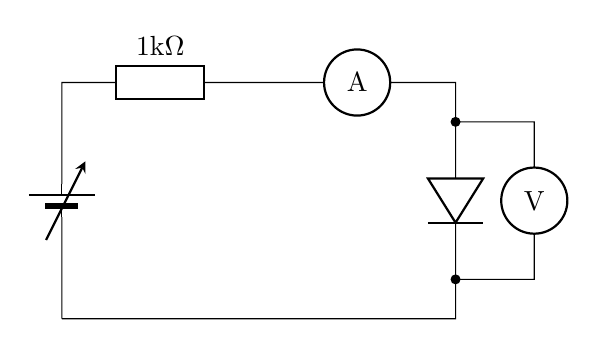
\begin{tikzpicture}% coordinates%\begin{}[]%\addplot coordinates {};%\end{}%\end{}
		% 電源・抵抗・電流計・ダイオード
		\draw (0,0)
		to [battery2] (0,3)
		to [european resistor = 1k$\Omega$] ++(2.5, 0)
		to [rmeter, t = A] ++(2.5,0)
		to [diode] ++(0,-3)
		to [short] (0,0)
		;
		% 電圧計
		\draw (5,0.5)
		to [short, *-] (6,0.5)
		to [rmeter, t = V] (6,2.5)
		to [short, -*] (5,2.5)
		;
		% 電源(可変矢印)
		\draw [->, >=stealth, thick] (-0.2,1)
		to (0.3,2)
		;
	\end{tikzpicture}
	\label{f5.5}
\end{figure}

\begin{figure}[H]
	\centering
	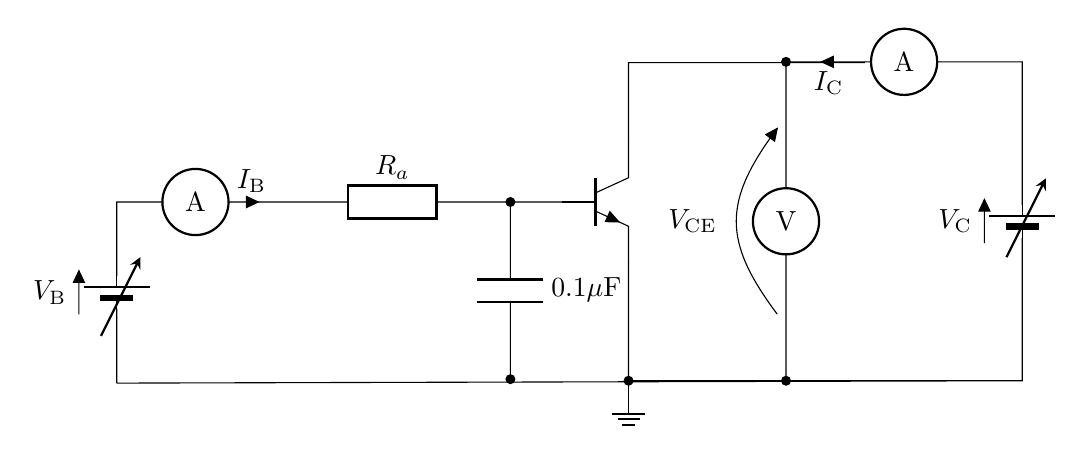
\begin{tikzpicture}% coordinates%\begin{}[]%\addplot coordinates {};%\end{}%\end{}
		% 電源・抵抗・電流計・ダイオード
		\draw (0,0)
		to [battery2 = $V_\mathrm{B}$] (0,2.3)
		to [rmeter, t = A, i=$I_\mathrm{B}$] ++(2,0)
		to [european resistor = $R_a$, -*] ++(3,0) coordinate(C1)
		to [short] ++(1,0) coordinate(a)
		(C1) to [C=$0.1\si{\mu F}$, -*] ++ (0,-2.25)
		(a) ++ (0.5,0) node [npn] (npn) {}
		(npn.C) -- ++ (0,1)
		to [short] ++ (3,0)
		(npn.E)
		to [short, -*] ++ (0,-1.5) node [ground] (ground) {}
		to [short] ++ (5,0) coordinate(right bottom)
		to [battery2 = $V_\mathrm{C}$] ++(0,4.05)
		to [rmeter, t = A, i = $I_\mathrm{C}$, -*] ++ (-3,0)
		to [rmeter, t = V, v = $V_\mathrm{CE}$, -*] ++ (0,-4.05)
		(right bottom)
		to [short] (0,0)
		;
		% 電源(可変矢印)
		\draw [->, >=stealth, thick]
		(-0.2,0.6) to (0.3,1.6)
		;
		\draw [->, >=stealth, thick]
		(11.3
		,1.6) to (11.8,2.6)
		;
	\end{tikzpicture}
	\label{f5.6}
\end{figure}


\begin{figure}[H]
	\centering
	\begin{circuitikz}
		\ctikzset{quadpoles/transformer core/inner=1, quadpoles/transformer core/width=0.6}
		\draw
			(0,-3) node [transformer core] (P) {}
			(P.A1) node [anchor=east] {}
			(P.A2) node [anchor=east] {}
			(P.B1) node [anchor=west] {}
			(P.B2) node [anchor=west] {}
			;
		% ==============
		%  電源
		% ==============
		\draw
			(P.A1) to [short] ++(-1,0) node [] (A1) {}
			(P.A2) to [short, *-] ++(-1,0) node [] (A2) {}
			(A1) to [sV] (A2)
			(A1) node [anchor=north east] {FG}
			;
		% ==============
		%  トランス右側縦
		% ==============
		\draw
			(P.B1) 
			to [short] ++(0,1) node [] (B1) {}
			to [short, -*] ++(2,0) node [] (D1) {}
			;
		\draw
			(P.B2) 
			to [short] ++(0,-2) node [] (B2) {}
			to [short, -*] ++(2,0) node [] (D2) {}
			;
		% ==============
		%  Z 回路
		% ==============
		\draw
			(D1) to [european resistor =$Z$, -*] ++(0,-2.6) node (GND) {} node [anchor=west] (CND) {GND}
			;
		% ==============
		%  R100
		% ==============
		\draw
			(GND) to [european resistor = $R_{100}$] (D2)
			;
		% ==============
		%  A2 to GND
		% ==============
		\draw
			(P.A2) to [short] ++(2,0)
			to [short] ++(0,0.5)
			(GND) to [short] ++(-0.84,0)
			;
	\end{circuitikz}
	\caption{$RZ$直列回路実験図}
	\label{EQUPZ}
\end{figure}

\begin{figure}[H]
	\centering
	\begin{circuitikz}
		\ctikzset{quadpoles/transformer core/inner=1, quadpoles/transformer core/width=0.6}
		\draw
			(0,-3) node [transformer core] (P) {}
			(P.A1) node [anchor=east] {}
			(P.A2) node [anchor=east] {}
			(P.B1) node [anchor=west] {}
			(P.B2) node [anchor=west] {}
			;
		% ==============
		%  電源
		% ==============
		\draw
			(P.A1) to [short] ++(-1,0) node [] (A1) {}
			(P.A2) to [short, *-] ++(-1,0) node [] (A2) {}
			(A1) to [sV] (A2)
			(A1) node [anchor=north east] {FG}
			;
		% ==============
		%  トランス右側縦
		% ==============
		\draw
			(P.B1) 
			to [short] ++(0,1) node [] (B1) {}
			to [short, -*] ++(2,0) node [] (D1) {}
			;
		\draw
			(P.B2) 
			to [short] ++(0,-2) node [] (B2) {}
			to [short, -*] ++(2,0) node [] (D2) {}
			;
		% ==============
		%  L回路
		% ==============
		\draw
			(D1) to [L=$L$, -*] ++(0,-2.6) node (GND) {} node [anchor=west] (CND) {GND}
			;
		% ==============
		%  R100
		% ==============
		\draw
			(GND) to [european resistor = $R_{100}$] (D2)
			;
		% ==============
		%  A2 to GND
		% ==============
		\draw
			(P.A2) to [short] ++(2,0)
			to [short] ++(0,0.5)
			(GND) to [short] ++(-0.84,0)
			;
	\end{circuitikz}
	\caption{$RL$直列回路実験図}
	\label{EQUPL}
\end{figure}

\begin{figure}[H]
	\centering
	\begin{circuitikz}
		\ctikzset{quadpoles/transformer core/inner=1, quadpoles/transformer core/width=0.6}
		\draw
			(0,-3) node [transformer core] (P) {}
			(P.A1) node [anchor=east] {}
			(P.A2) node [anchor=east] {}
			(P.B1) node [anchor=west] {}
			(P.B2) node [anchor=west] {}
			;
		% ==============
		%  電源
		% ==============
		\draw
			(P.A1) to [short] ++(-1,0) node [] (A1) {}
			(P.A2) to [short, *-] ++(-1,0) node [] (A2) {}
			(A1) to [sV] (A2)
			(A1) node [anchor=north east] {FG}
			;
		% ==============
		%  トランス右側縦
		% ==============
		\draw
			(P.B1) 
			to [short] ++(0,1) node [] (B1) {}
			to [short, -*] ++(2,0) node [] (D1) {}
			;
		\draw
			(P.B2) 
			to [short] ++(0,-2) node [] (B2) {}
			to [short, -*] ++(2,0) node [] (D2) {}
			;
		% ==============
		%  C回路
		% ==============
		\draw
			(D1) to [C=$C$, -*] ++(0,-2.6) node (GND) {} node [anchor=west] (CND) {GND}
			;
		% ==============
		%  R100
		% ==============
		\draw
			(GND) to [european resistor = $R_{100}$] (D2)
			;
		% ==============
		%  A2 to GND
		% ==============
		\draw
			(P.A2) to [short] ++(2,0)
			to [short] ++(0,0.5)
			(GND) to [short] ++(-0.84,0)
			;
	\end{circuitikz}
	\caption{$RC$直列回路実験図}
	\label{EQUPC}
\end{figure}


\begin{figure}[H]
	\centering
	\begin{circuitikz}
		\ctikzset{quadpoles/transformer core/inner=1, quadpoles/transformer core/width=0.6}
		\draw
			(0,-3) node [transformer core] (P) {}
			(P.A1) node [anchor=east] {}
			(P.A2) node [anchor=east] {}
			(P.B1) node [anchor=west] {}
			(P.B2) node [anchor=west] {}
			;
		% ==============
		%  電源
		% ==============
		\draw
			(P.A1) to [short] ++(-1,0) node [] (A1) {}
			(P.A2) to [short, *-] ++(-1,0) node [] (A2) {}
			(A1) to [sV] (A2)
			(A1) node [anchor=north east] {FG}
			;
		% ==============
		%  トランス右側縦
		% ==============
		\draw
			(P.B1) 
			to [short] ++(0,1) node [] (B1) {}
			to [short, -*] ++(2,0) node [] (D1) {}
			;
		\draw
			(P.B2) 
			to [short] ++(0,-2) node [] (B2) {}
			to [short, -*] ++(2,0) node [] (D2) {}
			;
		% ==============
		%  L回路
		% ==============
		\draw
			(D1) to [L=$L$, -*] ++(0,-2.6) node (GND) {} node [anchor=west] (CND) {GND}
			;
		% ==============
		%  R100
		% ==============
		\draw
			(GND) to [european resistor = $R_{100}$] (D2)
			;
		% ==============
		%  A2 to GND
		% ==============
		\draw
			(P.A2) to [short] ++(2,0)
			to [short] ++(0,0.5)
			(GND) to [short] ++(-0.84,0)
			;
	\end{circuitikz}
	\caption{$LC$直列回路実験図}
	\label{EQUP}
\end{figure}


\begin{figure}[H]
	\centering
	\begin{circuitikz}
		\ctikzset{quadpoles/transformer core/inner=1, quadpoles/transformer core/width=0.6}
		\draw
			(0,-3) node [transformer core] (P) {}
			(P.A1) node [anchor=east] {}
			(P.A2) node [anchor=east] {}
			(P.B1) node [anchor=west] {}
			(P.B2) node [anchor=west] {}
			;
		% ==============
		%  電源
		% ==============
		\draw
			(P.A1) to [short] ++(-1,0) node [] (A1) {}
			(P.A2) to [short, *-] ++(-1,0) node [] (A2) {}
			(A1) to [sV] (A2)
			(A1) node [anchor=north east] {FG}
			;
		% ==============
		%  トランス右側縦
		% ==============
		\draw
			(P.B1) 
			to [short] ++(0,1) node [] (B1) {}
			to [short, -*] ++(2,0) node [] (D1) {}
			;
		\draw
			(P.B2) 
			to [short] ++(0,-2) node [] (B2) {}
			to [short, -*] ++(2,0) node [] (D2) {}
			;
		% ==============
		%  C回路
		% ==============
		\draw
			(D1) to [C=$C$, -*] ++(0,-2.6) node (GND) {} node [anchor=west] (CND) {GND}
			;
		% ==============
		%  R100
		% ==============
		\draw
			(GND) to [european resistor = $R_{100}$] (D2)
			;
		% ==============
		%  A2 to GND
		% ==============
		\draw
			(P.A2) to [short] ++(2,0)
			to [short] ++(0,0.5)
			(GND) to [short] ++(-0.84,0)
			;
	\end{circuitikz}
	\caption{$LC$直列回路実験図}
	\label{EQUP}
\end{figure}

\begin{figure}[H]
	\centering
	\begin{circuitikz}[]
		\draw (0.5,2)
			to [short, o-*] (1,2)
			to [short] (1,3)
			to [european resistor=$R$] (3,3)
			to [L=$L$] (5,3)
			to [short, -*] (5,2)
			to [short] (5,1)
			to [C=$C$] (3,1)
			to [european resistor=$r$] (1,1)
			to [short] (1,2);
		\draw (5,2)	to [short, -o] (5.5,2);
	\end{circuitikz}
	\caption{ESRを考慮した並列共振回路}
	\label{ESR_P}
\end{figure}

\begin{figure}[H]
	\centering
	\begin{circuitikz}[]
		\draw (0,0) 
			node[transformer core] (T) {}
			(T.A1) node [anchor=east] {}
			(T.A2) node [anchor=east] {}
			(T.B1) node [anchor=west] {}
			(T.B2) node [anchor=west] {}
			(T.A1) to [sV] (T.A2)
			(T.B1) to [short] ++(0,1.5)
			to [short, -*] ++(1,0)
			to [L=$L$,] ++(0,-1.5) 
			to [C=$C$, -*] ++(0,-1.6) node[anchor=west] {GND}
			to [european resistor=$R_{100}$, -*] ++(0,-1.9)
			to [short] ++(-1,0)
			to [short] (T.B2)
			;
		\draw (T.A2) 
			to [short, -*] ++(0.63,0)
			to [short] ++(0.6,0)
			to [short] ++(0,0.5)
			to [short] ++(1.85,0)
			;
	\end{circuitikz}
	\caption{$LC$直列回路実験図}
	\label{EQUS}
\end{figure}

\begin{figure}[H]
	\centering
	\begin{circuitikz}
		\ctikzset{quadpoles/transformer core/inner=1, quadpoles/transformer core/width=0.6}
		\draw
			(0,-3) node [transformer core] (P) {}
			(P.A1) node [anchor=east] {}
			(P.A2) node [anchor=east] {}
			(P.B1) node [anchor=west] {}
			(P.B2) node [anchor=west] {}
			;
		% ==============
		%  電源
		% ==============
		\draw
			(P.A1) to [short] ++(-1,0) node [] (A1) {}
			(P.A2) to [short, *-] ++(-1,0) node [] (A2) {}
			(A1) to [sV] (A2)
			(A1) node [anchor=north east] {FG}
			;
		% ==============
		%  トランス右側縦
		% ==============
		\draw
			(P.B1) 
			to [short] ++(0,2) node [] (B1) {}
			to [short, -*] ++(2,0) node [] (D1) {}
			;
		\draw
			(P.B2) 
			to [short] ++(0,-2) node [] (B2) {}
			to [short, -*] ++(2,0) node [] (D2) {}
			;
		% ==============
		%  並列回路
		% ==============
		\draw
			(D1) to [short] ++(0,-0.8) node [] (C1) {}
			to [short] ++(0.5,0)
			to [L = $L$] ++(0,-2)
			to [short] ++(-0.5,0) node [] (C2) {}
			to [short] ++(-0.5,0)
			to [C = $C$] ++(0,2)
			to [short] ++(0.5,0)
			(C2) to [short, -*] ++(0,-0.8) node (GND) {} node [anchor=west] (CND) {GND}
			;
		% ==============
		%  R100
		% ==============
		\draw
			(GND) to [european resistor = $R_{100}$] (D2)
			;
		% ==============
		%  A2 to GND
		% ==============
		\draw
			(P.A2) to [short] ++(2,0)
			to [short] ++(0,0.5)
			(GND) to [short] ++(-0.84,0)
			;
	\end{circuitikz}
	\caption{$LC$直列回路実験図}
	\label{EQUP}
\end{figure}



\end{document}
